\section{Evolution of SBHS virtual labs}
In \cite{vlabs-kmm}, 
the control algorithm is implemented at the server end and the remote
student just keys in the parameters, as shown in Figure
\ref{fig:initial}. 
\begin{figure}
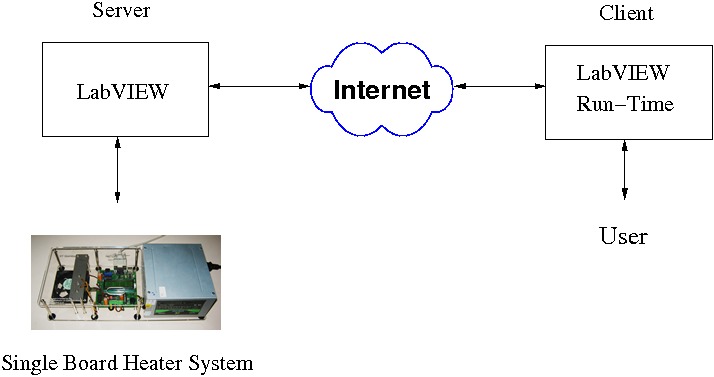
\includegraphics[width=\linewidth]{IEEE-Chile/figures/vlab-1.png}
\caption{SBHS virtual laboratory with remote access using LabVIEW}
\label{fig:initial}
\end{figure}
LabVIEW was used for the implementation of the same. The
server end consisted of a computer connected with an SBHS with a full
blown copy of LabVIEW installed on it. The client has a LabVIEW run
time engine available for free download from the National Instruments
website.  A few
LabVIEW algorithms/experiments were hosted on the server. The client
accesses these algorithm/experiment over the Internet using a web
browser by entering appropriate parameters.

It was realized that the learning experience is not complete for this
structure. This is because the server hosts some pre-built LabVIEW
algorithms and a user can only access these few algorithms. The user
can in no way change the program and can only input experimental
parameters. 
Hence, we came up with a new architecture
as shown in the Figure \ref{fig:second} that used full blown copies of
LabVIEW at both server and client ends.  
\begin{figure}
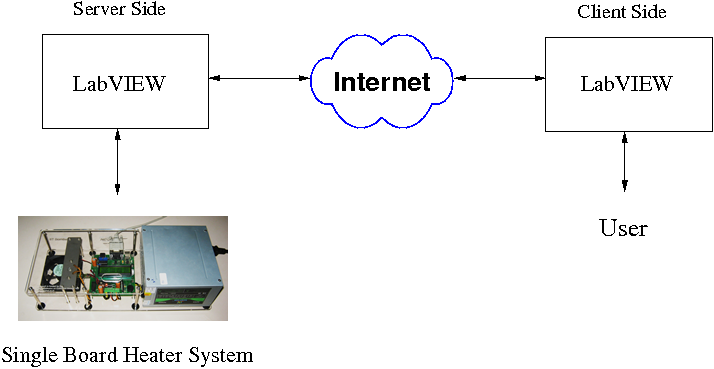
\includegraphics[width=\linewidth]{IEEE-Chile/figures/vlab-2.png}
\caption{SBHS virtual laboratory with remote access and live data sharing using LabVIEW}
\label{fig:second}
\end{figure}
 
 This idea uses the DataSocket technology of LabVIEW. Since now the
 client is having a complete LabVIEW installation on his/her computer
 she can now implement her own algorithms.  Thus this architecture did
 provide a complete learning experience to the students.  There are
 some shortcomings as well:

\begin{itemize}
\item LabVIEW is expensive and students may not be able to afford to
  buy it.  It is also prohibitively expensive for the Government to
  distribute it.

\item We used the LabVIEW version 8.04, which had restricted scripting
  language.  It was tedious to create new control algorithms in it.
\end{itemize}
\begin{figure}
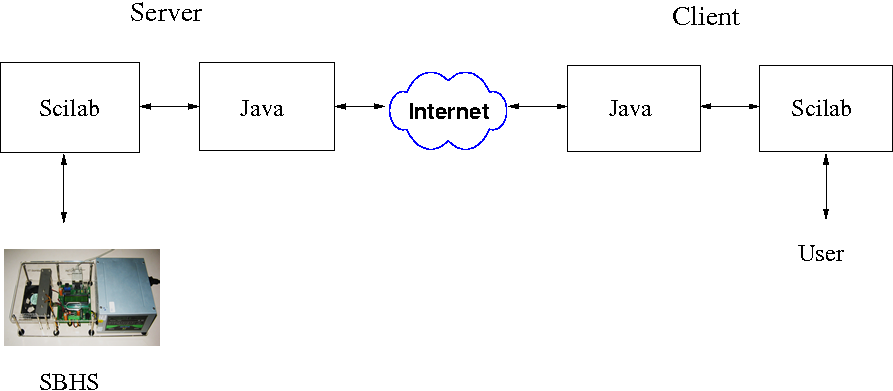
\includegraphics[width=\linewidth]{IEEE-Chile/figures/vlab-3.png}
\caption{SBHS virtual laboratory using open source software}
\label{fig:third}
\end{figure}
This made us shift to free and open source (FOSS) software. We
replaced LabVIEW with Java and Scilab as shown in Figure
\ref{fig:third}. Scilab at the server end is used for communicating
with SBHS. Scilab at the client end is used for implementing the
algorithms. Java is used at both the server as well as client end for
communication over the Internet thereby connecting the client with the
server. 

For the above solution, we need a dedicated copy of scilab running at
the server end for every SBHS. One way to do this is to host it on
multiple computers with unique IPs. Hence the number of SBHS we want
to host requires as many computer's and public IPs thereby making
it expensive. Moreover, it also limits its scalability. The other way
to do this is to host multiple java and scilab servers on the same
computer.  Hosting many copies of Scilab simultaneously requires a
powerful computer for the server.

For these reasons  we decided to take scilab off the server computer
and to use java alone to communicate with the SBHS directly.  Java
also 
communicates with the client computer.  We connected seven SBHS
systems to a USB port through a serial port hub.  This architecture
was 
implemented on a Windows Operating System.  We faced the following
difficulties in this solution.
\begin{itemize}
\item When we connected more than one serial hub to a PC, the port ID
  could not be retrieved correctly.  Port ID information is required
  if we want a student to use the same SBHS for all their experiments
  during different sessions.
\item The experiments required time stamping of the data communicated
  to and from the server. But this time stamping was not linear and
  suffered instability.  
\end{itemize}%
This made us to completely switch to FOSS with Ubuntu Linux as the OS
and is the current structure of the Virtual lab as shown in Figure
\ref{fig:detail-arch} 

\begin{figure}
\centering
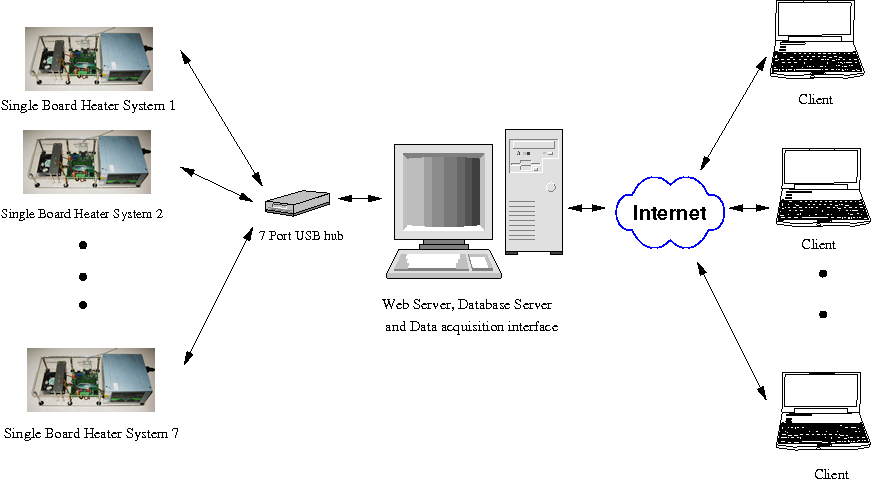
\includegraphics[width=\linewidth]{IEEE-Chile/figures/vlab-arch}
\caption{Virtual control lab hardware architecture}
\label{fig:hw-arch}
\end{figure}

\section{Current Hardware Architecture}
The current hardware architecture of the virtual single-board heater system lab involves 36 single-board heater systems connected to the server via multiple 7 and 10-port USB hubs. The server computer is connected to a high speed internetwork and has enough processing capability to host data acquisition, database, and web servers. 
It has been successfully tested for the undergraduate Process Control course and the graduate Digital Control and Embedded systems courses conducted at IIT Bombay as well as few workshops over the internet. Currently, this architecture is integrated with a cameras on each SBHS to facilitate live video streaming. This gives the user a feel of remote hands-on. 

\section{Current Software Architecture} \label{sec:vlabarchi}
The current software architecture of this virtual SBHS control lab is shown in Figure \ref{fig:detail-arch}. The server computer runs Ubuntu Linux 12.04.2 OS. It hosts a Apache-MySQL server. The SBHS server is based on Python-Django framework and is linked to Apache server using Apache's WSGI module. The MySQL database server has the details of all the registered users, their slot details, authentication keys to allow remote access, etc. As shown in Figure \ref{fig:sbhs-website}, the Python-Django server has pages for registration, login, slot booking etc. \cite{vl010}.  On the client end, control algorithms are running in Scilab and a python based client application communicates with virtual labs server over the Internet.



\begin{figure}
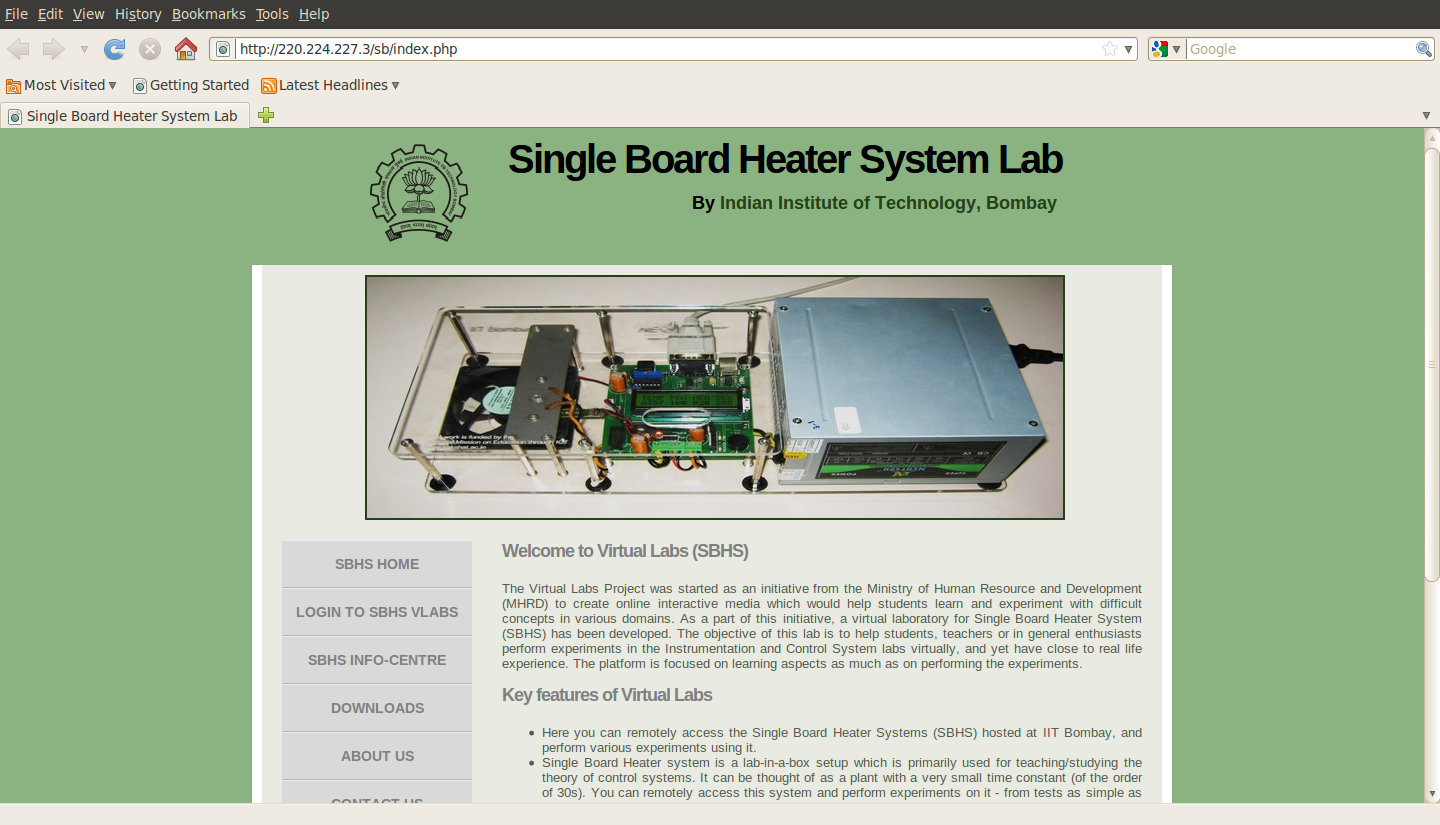
\includegraphics[width=\linewidth]{IEEE-Chile/figures/webpage}
\caption{Home page of SBHS V Labs}
\label{fig:sbhs-website}
\end{figure}
The steps to be performed before and during each experiment are explained next.

\begin{figure}
\centering
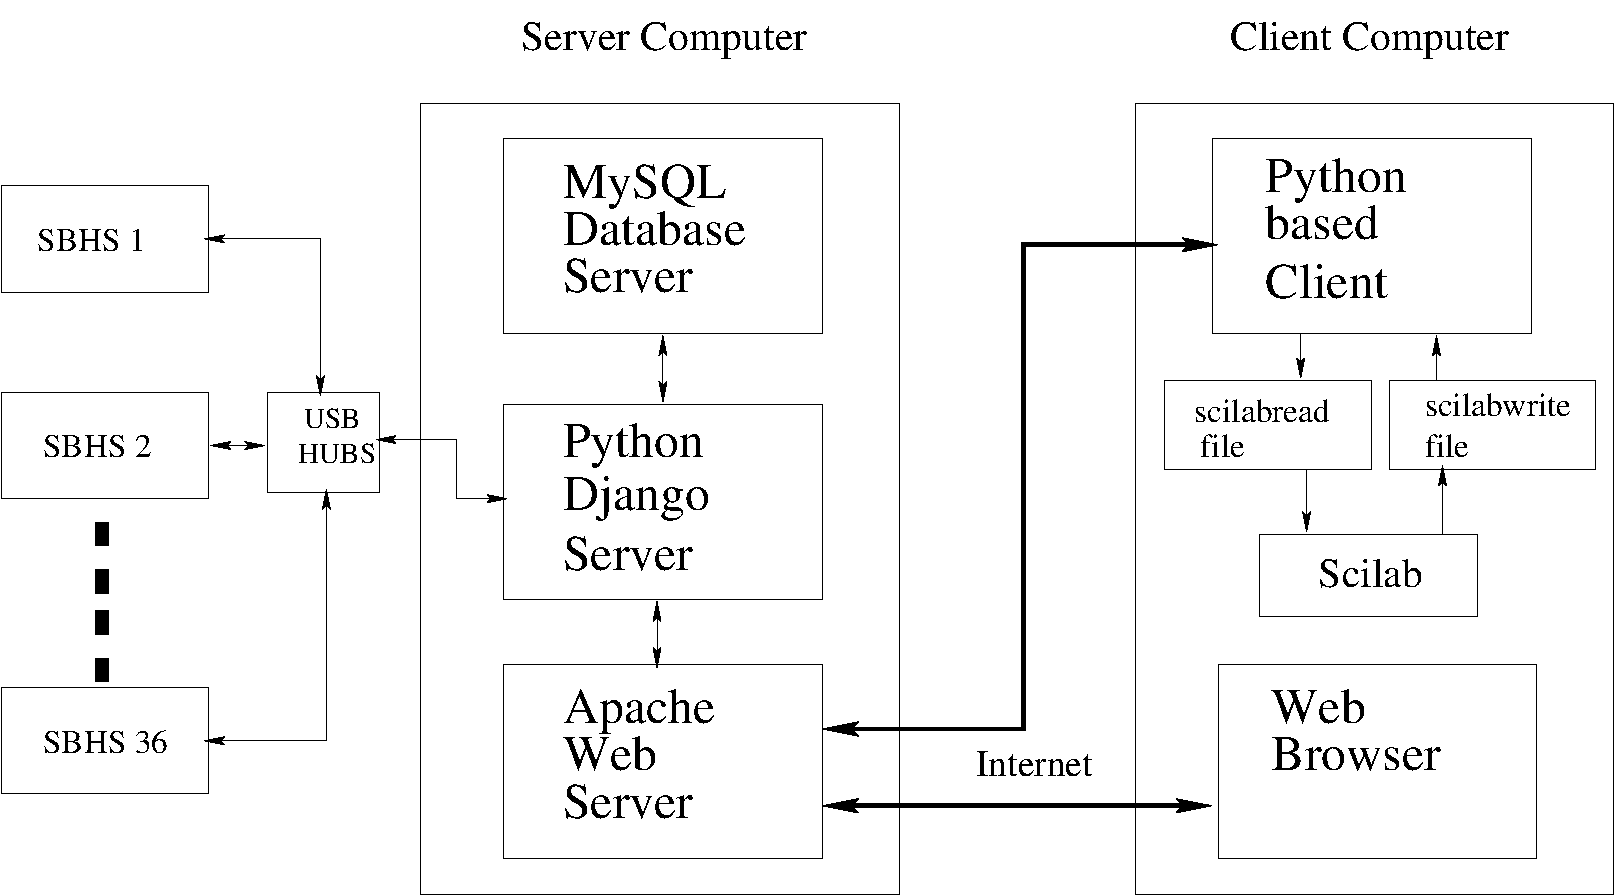
\includegraphics[width=\linewidth]{IEEE-Chile/figures/new-server-arch.pdf}
\caption{Current Architecture of SBHS Virtual Labs}
\label{fig:detail-arch}
\end{figure}





%\end{enumerate}






